Abbiamo visto che nelle interazioni devoli non viene conservato il sapore dei quark. Questo è associato a transizione con scambio di carica dei quark. Ad esempio nella trasformazione di un protone in un neutrone abbiamo un quark up che si trasforma in un quark down. Spesso associate a produzioni di coppie leptone-neutrino, ma anche coppie di quark-antiquark, di carica diversa. Queste caratteristiche permettono il prodursi di un fenomeno spettacolare: il fatto che le interazioni deboli non conservino il sapore significa che gli autostati dell'hamiltoniana globale non necessariamente consevrano il sapore, quindi gli autostati dell'hamiltoniana globale possono non essere autostati di sapore. In particolare quello che abbiamo sono le oscillazioni tra una particella e la sua antiparticella. Introdurremo una Hamiltoniana efficace che include la descrizione degli autostati, la loro evoluzione temporale ed il decadimento. Questo fenomeno ha permesso di osservare la violazione di CP.
\subsection{Violazione di CP}
La violazione di CP è fondamentale per diversi motivi: \textbf{asimmetria materia-antimatieria nell'universo} e dal fatto dell'esistenza di una \textbf{freccia del tempo}. Sul primo punto abbiamo evidenziato che nell'universo contenga molti più barioni e elettroni che anti-barioni e positroni. Ammontare osservato nei raggi cosmici compatibile con i processi di spallazione, conversione di coppie ed altri. Perchè possa generarsi questa asimmetria è necessario soddisfare le tre condizioni di Sakharov (1967): deve esistere un processo che violi il numero barionico, devono essere violare C e CP e tali processi devono avvenire al di fuori dall'equilibrio termico.

Per la freccia del tempo si ha che noi crediamo che CPT sia una simmetria fondamentale della natura. La violazione di CP e conservazione di CPT implicano violazione di T. \textbf{Invarianza per invesione temporale rotta a livello microscopico}.
\subsection{I decadimenti dei quark}
I quark possono essere classificati in famiglie, come i leptoni. Ci sono due famiglie di carica: i quark con carica $Q=+2/3$ e carica $Q=-1/3$. Questi quark si possono vedere in collisioni perchè quando vado all'energia giusta per uno stato legato quark e antiquark abbiamo degli stati di risonanza. Le transizioni deboli sono mediate dalla matrice \textbf{unitaria} di Cabibbo-Kobayashi-Maskawa (CKM):
\begin{equation*}
    \begin{pmatrix} V_{ud} & V_{us} & V_{ub} \\ V_{cd} &
V_{cs} & V_{cb} \\ V_{td} & V_{ts} &
V_{tb}\end{pmatrix}\approx\begin{pmatrix} \cos{\theta_{C}} & \sin{\theta_{C}} & \sim10^{-3} \\ -\sin{\theta_{C}} &
\cos{\theta_{C}} & \sim10^{-2} \\ \sim10^{-3} & \sim10^{-2} &
1\end{pmatrix}
\end{equation*}
Esempio un quark s si può trasformare in:
\begin{equation*}
    |s\rangle\to V_{us}|u\rangle+\cancel{V_{cs}|c\rangle}+\cancel{V_{ts}|t\rangle}
\end{equation*}
E un quark c invece:
\begin{equation*}
    |c\rangle\to V^*_{cd}|d\rangle+V^*_{cs}|s\rangle+\cancel{V^*_{cb}|b\rangle}
\end{equation*}
Non tutti i decadimenti sono possibili cinematicamente. Per cui per esempio il decadimento delle particelle strane fosse con una costante $G$ di un'ordine di grandezza più bassa della costante $G_F$. Questo è dovuto al fatto che $s$ può decadere in $c$ e $t$ ma questi decadimenti non sono permessi cinematicamente per cui solo la funzione d'onda proporzionale al $\sin{\theta_c}$. Quindi per esempio abbiamo certe interazioni proporzionali a cose diverse. La cosa interessante è che in queste transizioni avvengono mediate da un bosone vettore che è carico $W$. Questo $W$ porta via il $Q$ valore di questa reazione e questa energia è disponibile per produrre leptone e il suo anti-neutrino nei decadimenti $\beta$ oppure quark e anti-quark nei decadimenti adronici.

IL Q valore viene usato per produrre coppie $lv$ o $qq$ entro il range delle interazioni deboli (dalla teoria di Yukawa):
\begin{equation*}
    \frac{\hbar}{m_Wc^2}\sim2.5\times10^{-3}fm
\end{equation*}
\subsection{Oscillazioni particella-antiparticella}
L'osservazione principale è che il "sapore" dei quark non è una quantità esattamente conservata. Viene conservata nelle interazioni forti ed elettromagnetiche. Per cui abbiamo visto che possiamo avere dei decadimenti elettromagnetici della $\Sigma$ in $\Lambda$ perchè conservano la stranezza. Questo non avviene però nelle interazioni deboli. Alcuni stati mesonici neutri come:
\begin{equation*}
    K^0(d\Bar{s})\leftrightarrow\Bar{K}^0(\Bar{d}s) \qquad B_d^0(d\Bar{b})\leftrightarrow\Bar{B}_d^0(\Bar{d}b)
\end{equation*}
Questi stati la particella e l'antiparticella differiscono solamente per il numero quantico di sapore (stranezza, bellezza, $\ldots$), che però non è conservato nelle interazioni deboli. Per cui non essendo conservato non ho nessuna quantità conservata che non mi obbliga nel passara dalla particella alla sua antiparticella. \textbf{Autostati di sapore non sono, in generale, autostati dell'Hamiltoniana}. Nota bene: non sono possibili altre oscillazioni di particelle neutre. Ad esempio l'oscillazione neutrone-antineutrone, visto che le due particelle hanno diverso numero barionico, ed il numero barionico è conservato. Lo stesso non ho oscillazioni neutrino-antineutrino visto che le due particelle hanno diverso numero leptonico, che pure è una quantità conservata. Importante il collegamento quantità conservata e simmetria dell'interazione.
\subsection{Hamiltoniana efficace}
Vediamo ora come possiamo descrivere la cosa dal punto di vista matematico. Nel caso di particella in quiete:
\begin{equation*}
    E=m
\end{equation*}
l'equazione di Schr\"odinger:
\begin{equation*}
    i\frac{d}{dt}\psi=m\psi
\end{equation*}
dove $H\psi=m\psi$ con $m=\langle \psi|H|\psi\rangle$. La sua evoluzione temporale sarà:
\begin{equation*}
    \psi(t)=\psi(0)e^{-imt}
\end{equation*}
e la densità di probabilità:
\begin{equation*}
    |\psi(t)|^2=|\psi(0)|^2=\text{costante}
\end{equation*}
Se la particella è \textbf{instabile} si può descrivere con una componente \textbf{immaginaria} dell'autovalore dell'energia:
\begin{equation*}
    H\psi=\left(m-i\frac{\gamma}{2}\right)\psi
\end{equation*}
ora vedo che l'evoluzione temporale diventa:
\begin{equation*}
    \psi(t)=\psi(0)e^{-imt-\frac{\gamma}{2}t}
\end{equation*}
E la densità di probabilità decresce nel tempo:
\begin{equation*}
    |\psi(t)|^2=|\psi(0)|^2e^{-\gamma t}
\end{equation*}
$H$ non è hermitiana in quanto non conserva la densità di probabilità: descrive in maniera efficace il comportamento di un singolo stato di un sistema più ampio. Dove $\gamma$ è la larghezza di decadimento dello stato.
\subsubsection{Sistema del Kzero}
Consideriamo il caso dei due stati del $K^0$ e della sua antiparticella:
\begin{equation*}
    \psi(t)=a(t)|K^0\rangle+b(t)|\Bar{K}^0\rangle
\end{equation*}
\begin{equation*}
    i \frac{d}{d t} \psi(t)=i \frac{d}{d t} a(t)\left|K^0\right\rangle+i \frac{d}{d t} b(t)\left|\bar{K}^0\right\rangle=H \psi(t)=a(t) H\left|K^0\right\rangle+b(t) H\left|\bar{K}^0\right\rangle
\end{equation*}
Facendo il prodotto scalare con $\langle K^0|$:

\begin{equation*}
    i \frac{d}{d t} a(t) =a(t)\left\langle K^0|H| K^0\right\rangle+b(t)\left\langle K^0|H| \bar{K}^0\right\rangle
\end{equation*}
Facendo il prodotto scalare con $\langle \Bar{K}^0|$:
\begin{equation*}
    i \frac{d}{d t} b(t) =a(t)\left\langle\bar{K}^0|H| K^0\right\rangle+b(t)\left\langle\bar{K}^0|H| \bar{K}^0\right\rangle 
\end{equation*}
possiamo scrivere in forma matriciale:
\begin{equation*}
    i \frac{d}{d t}\left(\begin{array}{c} a(t) \\ b(t) \end{array}\right)=\left(\begin{array}{cc} \left\langle K^0|H| K^0\right\rangle & \left\langle K^0|H| \bar{K}^0\right\rangle \\ \left\langle\bar{K}^0|H| K^0\right\rangle & \left\langle\bar{K}^0|H| \bar{K}^0\right\rangle \end{array}\right)\left(\begin{array}{c} a(t) \\ b(t) \end{array}\right)=H_{e f f}\left(\begin{array}{c} a(t) \\ b(t) \end{array}\right)
\end{equation*}
Se esistessero solo interazioni elettromagnetiche e forti: per la conservazione della stranezza
\begin{equation*}
    \left\langle K^0|H| \bar{K}^0\right\rangle=\left\langle \bar{K}^0|H| K^0\right\rangle
\end{equation*}
per la simmetria di coniugazione di carica: i due elementi devono essere uguali ed essere reali perchè mi impedisce il decadimento del $K^0$
\begin{equation*}
    \left\langle K^0|H| K^0\right\rangle=\left\langle \Bar{K}^0|H| \Bar{K}^0\right\rangle=m_{K^0}
\end{equation*}
\subsection{Hamiltoniana efficace}
La forma più generale dell'hamiltoniana efficace si può ottenere scomponendola in una parte hermitiana ed una anti-hermitiana:
\begin{equation*}
    H_{eff}=M-i\frac{\Gamma}{2}=\begin{pmatrix} m_0 & m_{12} \\ m^*_{12} & m_0 \end{pmatrix}-i\frac{1}{2}\begin{pmatrix} \Gamma_0 & \Gamma_{12} \\ \Gamma^*_{12} & \Gamma_0 \end{pmatrix}
\end{equation*}
Dove $M$ e $\Gamma$ sono matrici hermitiane. e abbiamo indicato:
\begin{equation*}
    \left\langle K^0|H| K^0\right\rangle=\left\langle \Bar{K}^0|H| \Bar{K}^0\right\rangle=m_0-i\frac{\Gamma_0}{2}
\end{equation*}
Si può dimostrare che la conservazione di CPT impone:
\begin{equation*}
    \left\langle K^0|H| K^0\right\rangle=\left\langle \Bar{K}^0|H| \Bar{K}^0\right\rangle
\end{equation*}
Mostreremo che se $m_{12}$ e $\Gamma_{12}$ sono reali, allora $H_{eff}$ conserva CP. Se ci fossero solo interazioni forti ed elettromagnetiche:
\begin{equation*}
    H_{eff}=m_{K^0}\begin{pmatrix} 1 & 0 \\ 0 & 1 \end{pmatrix} \qquad \psi(t)=\psi(0)\exp(-im_{K^0}t)
\end{equation*}
\subsubsection{Oscillazioni: visione microscopica}
Le interazioni deboli: permettendo che il decadimento producono una componente immaginaria negli autovalori, le modifiche della stranezza avvengono tramite scambi multipli di $W$ (particella mediatrice) (mi trasforma il quark strano in qualcos'altro). 
%IMMAGINE ewe
\begin{figure}[htp!]
  \centering
  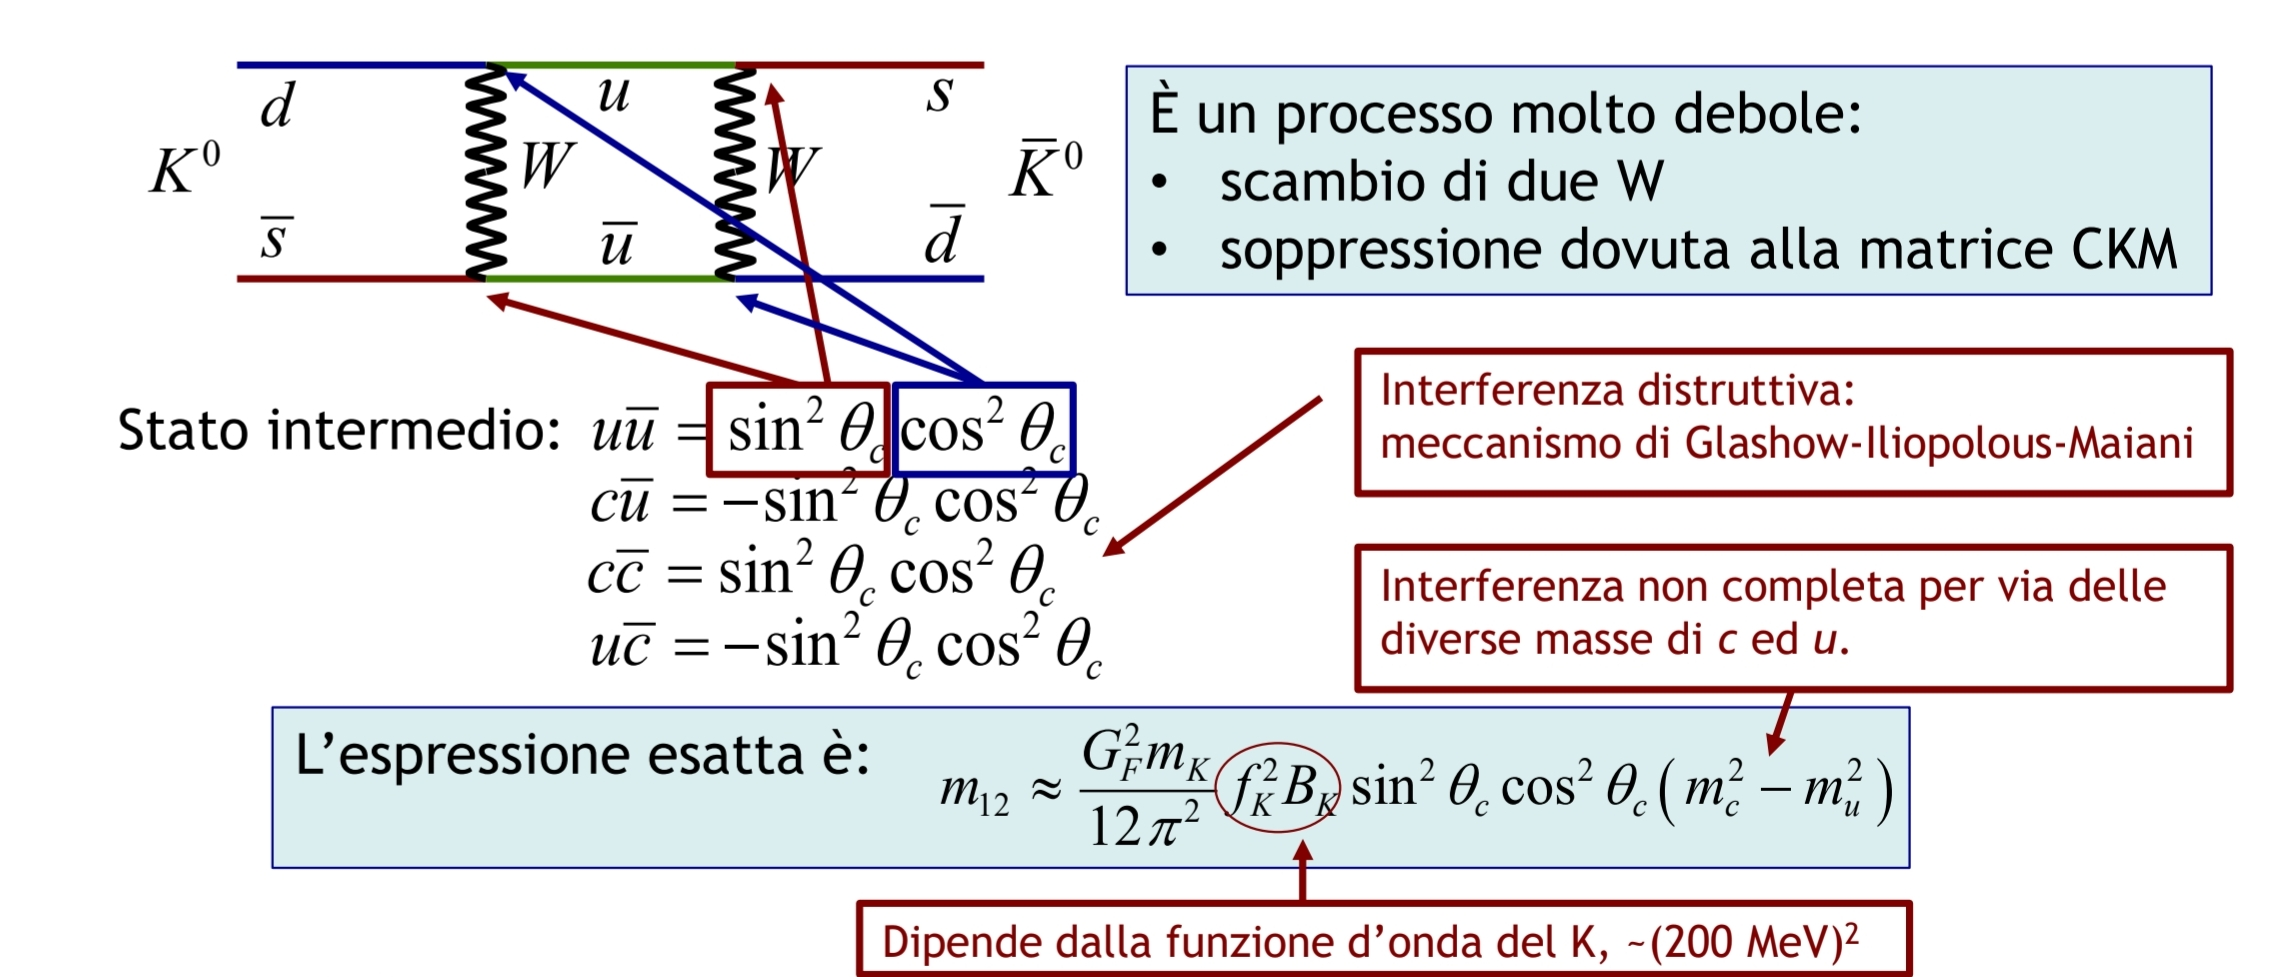
\includegraphics[scale=0.17]{Lezione17/ewe.jpg} 
\end{figure}
Per esempio un'interazione che posso avere è che se parto da un $K^0$ con un quark $d$ e un quark $\Bar{s}$. Quello che posso avere è che il quark $d$ si trasformi in un $u$ emettendo un $W$ che poi verrà assorbito dal quark $\Bar{s}$ per poi trasformarsi in $\Bar{u}$. Questo quark $u$ può emettere un altro $W$ e trasformarsi in un quark $s$ e allo stesso modo verrà assorbito da $\Bar{u}$ trasformandosi in $\Bar{d}$ ottenendo alla fine un $\Bar{K}^0$. A livello microscopico posso trasformare un $K^0$ in un $\Bar{K}^0$ attraverso scambi multipli di bosoni $W$. Questo è un processo davvero debole! è già faticoso scambiare un solo bosone $W$, quando si è conforntata l'intensità delle interazioni veniva che le interazioni deboli erano devboli perchè nell'elemento di matrice compariva un termine $(1/m_W)^2$ che dopo con il modulo quadro diventava ancora più potente faceva crollare drasticamente l'intensità della interazione. Oltre a questo c'è una ulteriore soppressione dovuta alla matrice CKM. Se pensiamo quali sono i pesi di questa interazioni. Questo stato stato intermedio non è l'unico che può avvenire per andare da $K^0$ a $\Bar{K}^0$. Si possono fare con i vari stati intermedi. Abbiamo quindi un'interferenza distruttiva tra questi stati intermedi perchè compaiono con segni diversi. Questo processo è detto meccanismo di Glashow-Ilipolous-Maiani. 
\subsubsection{Oscillazioni: visione macroscopica}
Si può arrivare allo stesso risultato qualitativo guardando gli stati di decadimento. Il fatto che ci possano essere termini non diagonali $m_{12}$ si può anche inferire dal fatto che ci sono decadimenti comuni a $K^0$ e $\Bar{K}^0$. Consideriamo i principali decadimenti dei $K$ carichi che non possono avere decadimenti comuni:
%IMMAGINE ewe
\begin{figure}[htp!]
  \centering
  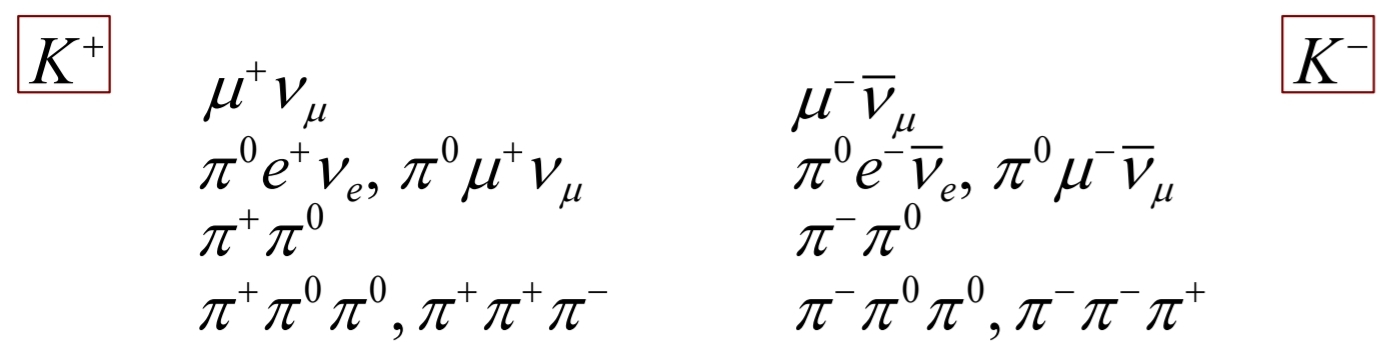
\includegraphics[scale=0.2]{Lezione17/tt.jpg} 
\end{figure}
Nella prima riga possiamo vedere decadimenti puramente leptonici come per il pione. C'è anche quello con l'elettrone anche se sarà difficile da produrre. Oppure nella seconda riga decadimenti analoghi a quelli $\beta$. Nella terza riga invece decadimenti in due pioni. Tecnincamente anche con tre pioni ma hanno un rapporto di decadimento piccolo. La carica è diversa quindi i due decadimenti sono diversi. Se invece prendo i $K$ neutri:
%IMMAGINE uu
\begin{figure}[htp!]
  \centering
  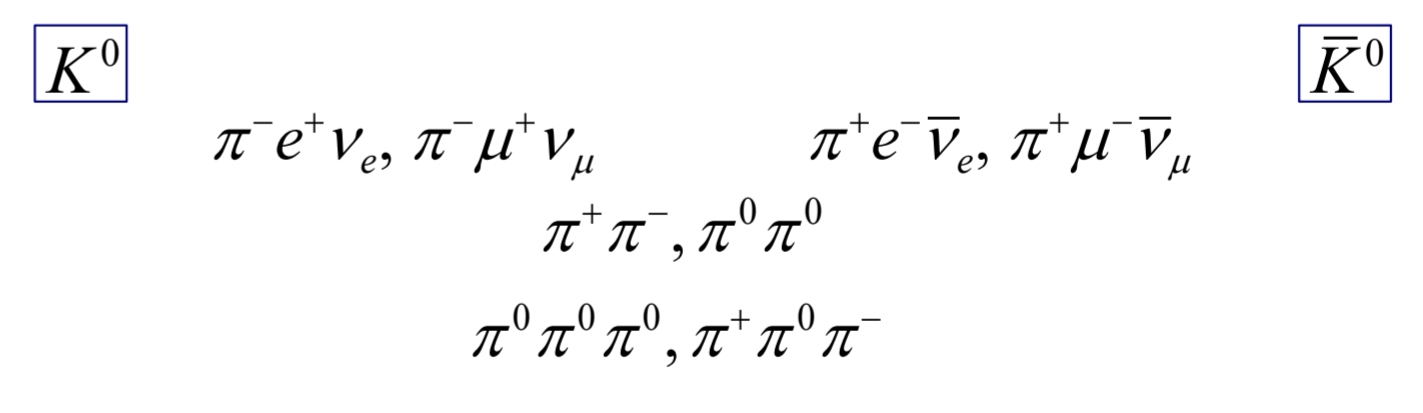
\includegraphics[scale=0.2]{Lezione17/uu.jpg} 
\end{figure}
Anche questi qua hanno decadimenti $\beta$ in cui però il $K^0$ mi decade in pione negativo e positrone mentre il $\Bar{K}^0$ in pione positivo ed elettrone. Questo perchè nel $K^0$ ho un $\Bar{s}$ che si trasforma in un $\Bar{u}$ e nel $\Bar{K^0}$ ho un $s$ che si trasforma in $u$ e quindi il muone che partecipa all'interazione ha diversa carica. Nel decadimento in due pioni questo solitamente sono coppie di pione positivo e negativo o due pioni neutri. E questi sono indistinguibili. Guardando questa coppia non posso sapere se arrivano da $K^0$ o $\Bar{K}^0$. La stessa cosa per il decadimento in tre pioni. Questa esistenza di stati in comune è molto importante. La presenza di stati comuni, infatti, implica che gli autostati dell'hamiltoniana completa devono essere misture di $|\Bar{K}^0\rangle$ e $|\Bar{K}^0\rangle$. Si torna alla teoria delle perturbazione in meccanica quantistica: Questo è analogo a quanto accade in una teoria con una hamiltoniana non relativistica H, con autofunzioni $\psi_n$: se aggiungiamo una perturbazione $V$, vediamo che le autofunzioni diventano:
\begin{equation*}
    \psi'_n=\psi_n+\sum_{m\ne n}\frac{\langle \psi_m|H|\psi_n\rangle}{E_n-E_m}\psi_m
\end{equation*}
Al primo ordine solo le le autofunzioni sono collegate direttamente contribuiscono. Al secondo ordine:
\begin{equation*}
    +\sum_{m \neq n} \sum_{k \neq n} \frac{\left\langle\psi_m|V| \psi_k\right\rangle\left\langle\psi_k|V| \psi_n\right\rangle}{\left(E_n-E_m\right)\left(E_n-E_k\right)} \psi_m-\sum_{m \neq n} \frac{\left\langle\psi_n|V| \psi_n\right\rangle\left\langle\psi_m|V| \psi_n\right\rangle}{\left(E_n-E_m\right)^2} \psi_m-\frac{\psi_n}{2} \sum_{m \neq n} \frac{\left|\left\langle\psi_m|V| \psi_n\right\rangle\right|^2}{\left(E_n-E_m\right)^2}
\end{equation*}
al secondo ordine contribuiscono anche autofunzioni collegate tramite uno stato a $\psi_k$ con prodotto $\ne0$ sia con $\psi_n$ e $\psi_m$. In particolare per la matrice $\Gamma$, intuitivamente possiamo dire che:
\begin{equation*}
    \Gamma_0=\frac{2\pi}{\hbar}\sum_f\langle K^0|H|f\rangle\langle f|H|K^0\rangle\rho_f \quad \Rightarrow\quad \Gamma_{12}=\frac{2\pi}{\hbar}\sum_f\langle \Bar{K}^0|H|f\rangle\langle f|H|K^0\rangle\rho_f
\end{equation*}
Dove il braket è l'elemento di matrice: $|M_{fK^0}|^2$.
\subsection{Diagonalizzazione di H efficace}
Ora che abbiamo una Hamiltoniana efficace possiamo chiederci quali sono gli autostati. Procederemo ora a determinare gli autovalori e autovettore di $H_{eff}$:
\begin{equation*}
    H_{eff}\begin{pmatrix}
        m_0-\frac{i}{2}\Gamma_0 & m_{12}-\frac{i}{2}\Gamma_{12} \\ m^*_{12}-\frac{i}{2}\Gamma^*_{12} & m_0-\frac{i}{2}\Gamma_0
    \end{pmatrix} \qquad |K_S\rangle=p|K^0\rangle+q|\Bar{K}^0\rangle \quad |K_L\rangle=p|K^0\rangle-q|\Bar{K}^0\rangle
\end{equation*}
Prima di procedere con i calcoli formali, anticipiamo i risultati principali: se $H_{eff}$ conserva CP (quindi non ci sono termini complessi), gli autostati sono gli autostati di CP:
\begin{equation*}
    |K_1\rangle=\frac{1}{\sqrt{2}}(|K^0\rangle-|\Bar{K}^0\rangle), \quad |K_2\rangle=\frac{1}{\sqrt{2}}(|K^0\rangle+|\Bar{K}^0\rangle)
\end{equation*}
Questi hanno una \textbf{grossa differenza di vita media}, dando luogo agli stati $K_S\sim K_1$ e $K_L\sim K_2$. L'interferenza di questi stati permette di osservare oscillazioni $|K^0\rangle\Leftrightarrow|\Bar{K}^0\rangle$. Nel 1964 Fitch e Cronin osservarono il decadimento $K^0_L$, CP dispari, in uno stato con CP pari: questo significa che $K^0_L$ non è un autostato di CP e inoltre è presente una violazione della simmetria CP nelle interazioni deboli. [slide per i calcoli]